% \Huge

\section{Cosmological Context}

\todo[inline]{Introduce the context of Modern Cosmology}

\section{The Cosmic Microwave Background}

\todo[inline]{Introduce the CMB and talk about the starting point. E.g.\ very smooth initial field with some anisotropies that will be locked in the matter distribution.}

\todo[inline]{Introduce BAOs.}

\begin{figure}
    \centering
    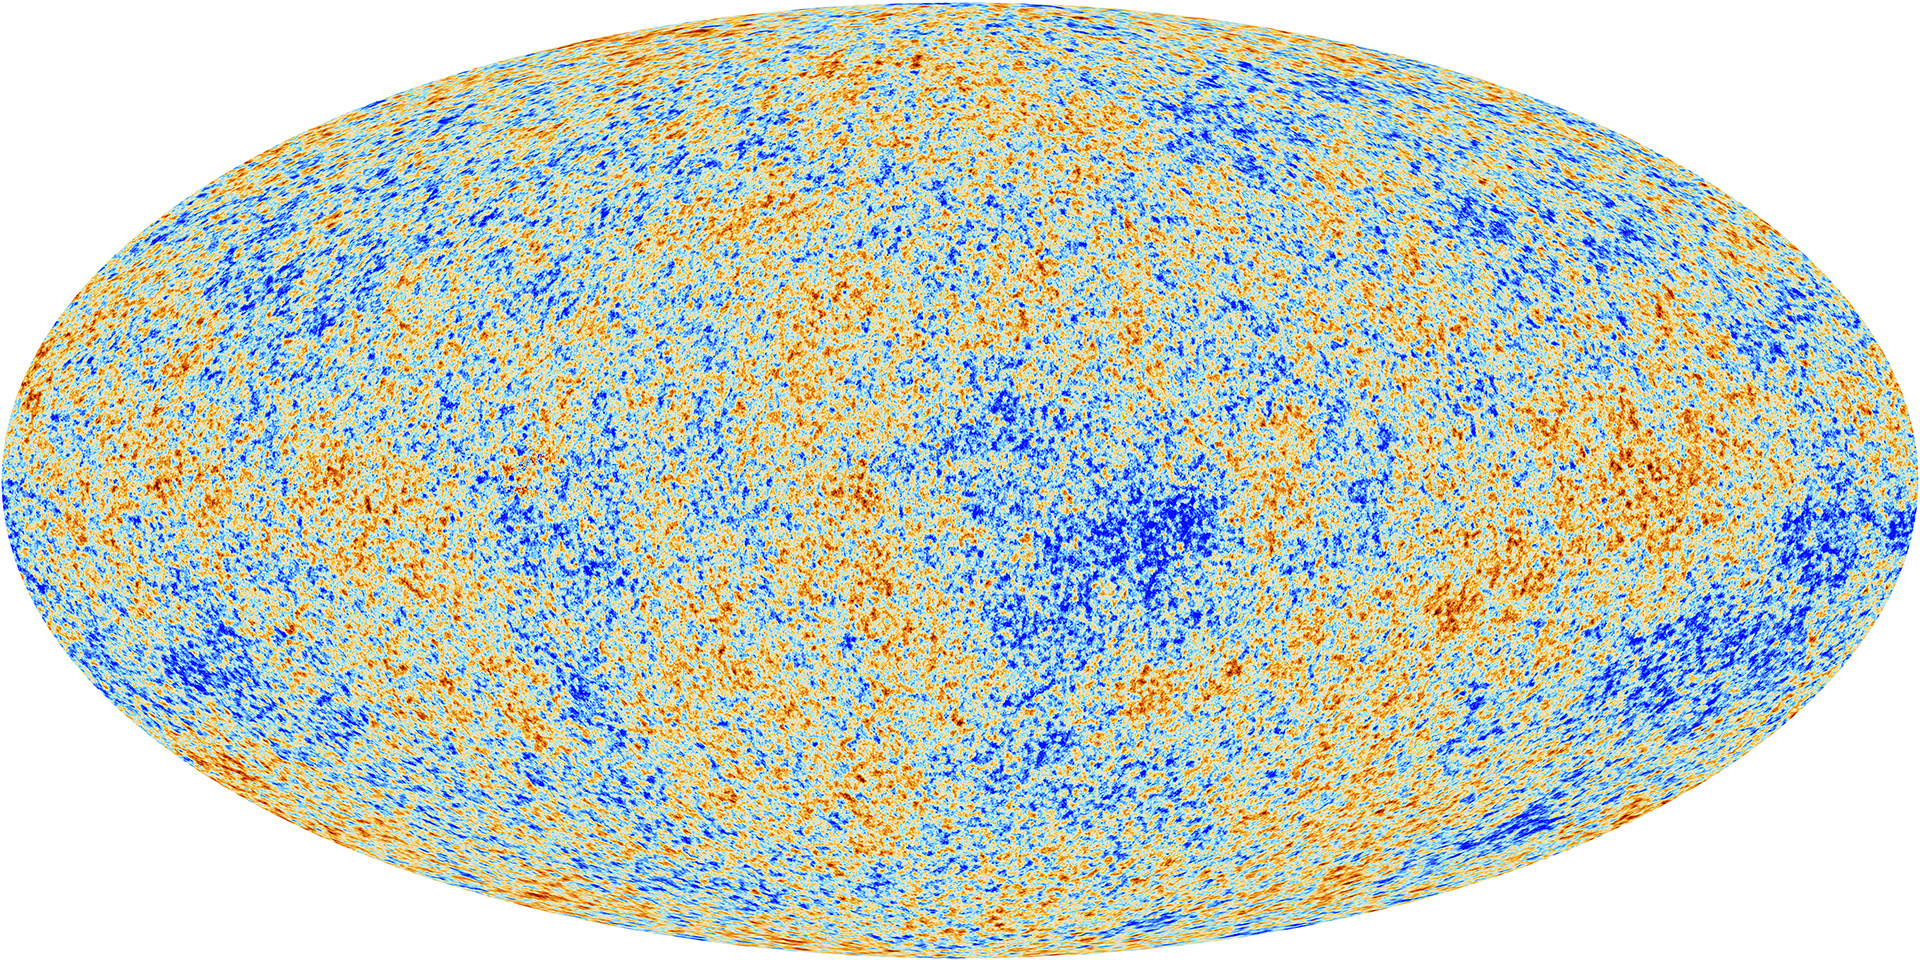
\includegraphics[width=0.9\columnwidth]{images/misc/Planck_CMB.jpg}%
    
    \caption{
    Map of the Cosmic Microwave Background aquired by the Planck Space Telescope (ref). 
    }
    
    \label{fig:1}
\end{figure}


\section{Large Scale Structure and Galaxy Surveys}

\todo[inline]{Introduce the Structure of the Universe today and the tools used to study it.}

\todo[inline]{Talk about the detection of the BAO in the galaxy distribution and its smearing due to collapse.}

\begin{figure}
    \centering
    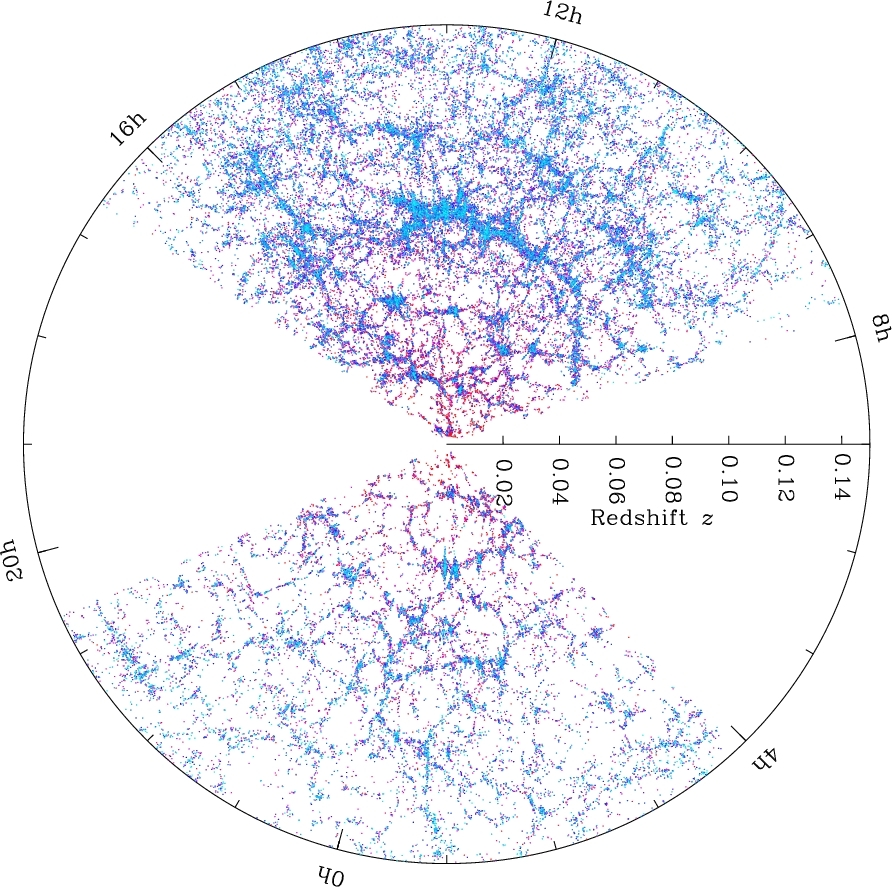
\includegraphics[width=0.9\columnwidth]{images/misc/orangepie.jpg}%
    
    \caption{
    Galaxy map from the Sloan Digital Sky Survey.
    }
    
    \label{fig:2}
\end{figure}


\section{The Missing Link (Reconstruction)}

\todo[inline]{Motivate our desire to link the two and talk about the problems we have (Dark Ages)}

\todo[inline]{Motivate the desire to reconstruct the BAO feature}
